\chapter*{Part B:\@ Approximation}

\section*{Introduction}

The California Housing data set consists of information collected from
the 1990 Census conducted by the United States Census Bureau. More
specifically, the data set focused on the median housing prices and 8
independent variables associated with the housing price for all the
block groups in California.

A block group is the smallest geographical unit for which the United
States Census Bureau publishes data. The geographical size of block
groups vary inversely with their population density, and they usually
have a population size of 600 to 3000 people. 

The entire data set has 20640 lines of data, and the variables
(listed in order) are:

\begin{itemize}
    \item Longitude
    \item Latitude
    \item Housing Median Age 
    \item Total Rooms
    \item Total Bedrooms
    \item Population
    \item Households
    \item Median Income
    \item Median House Value
\end{itemize}

The longitudes and latitudes were calculated from the centroids of each
block group, and any block groups that did not have statistics for one
or more variables were excluded from the final data set.

The aim of this part of the project is to predict the median housing price
of a block group, given the other 8 variables as input --- a regression
problem. The data was split into train and test sets, with each having 14322
and 6138 lines respectively (7:3 ratio). The train set was further split
into 5 parts to perform 5-fold cross-validation on the models tested, with
the final accuracy of the selected model obtained from testing with the
test set.

The use of multilayer feedforward networks to solve nonlinear regression
problems like these has been well documented. The only difference between
using these networks for classification problems and regression problems
is simply the activation function used in the output neuron\,(s). As such,
neural networks perform similarly well on regression problems.

\section*{Experiments}

We implemented the neural network as two functions \texttt{train\_test\,()}
and \texttt{cross\_validation\,()}, each
taking two optional parameters: \texttt{learning\_rate} and
\texttt{no\_hidden} (the hidden layer neuron count).
Each experiment is performed by utilizing the search function
\texttt{search\,()}, which takes two additional inputs, the search parameter
(either \texttt{learning\_rate} or \texttt{no\_hidden}) and the
search space associated with it. Depending on the flags set, the function
would either loop through the possible values of the parameter and perform
cross-validation on the training set, or train and test the neural
network on the whole data set. Graphs are stored and displayed after
each experiment.

\subsection*{Experiment 1: Building the reference 3-layer network (Question 1)}

Plotting the training errors against the number of epochs:

\begin{center}
    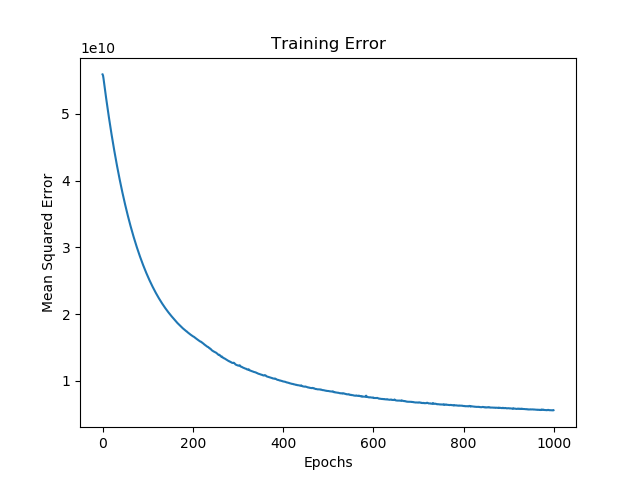
\includegraphics[width=\imgw]{images/p1b1_sample_train.png}   
\end{center}

Plotting the test errors against the number of epochs:

\begin{center}
    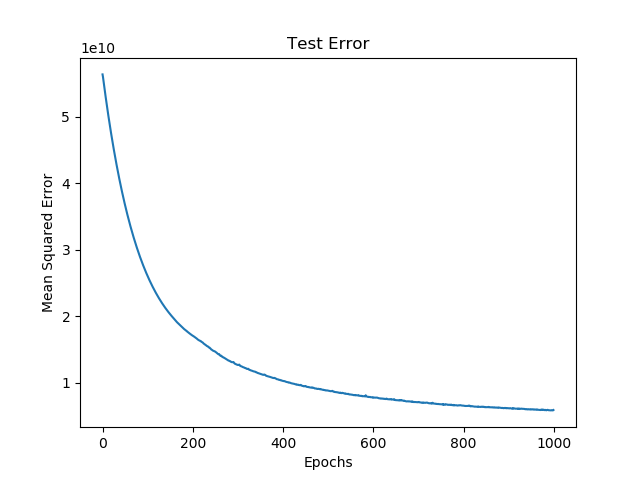
\includegraphics[width=\imgw]{images/p1b1_sample_test.png}   
\end{center}

\subsection*{Experiment 2: Determining the optimal learning rate
(Question 2)}

The parameter \texttt{learning\_rate} is varied in the search space
\([10^{-5},0.5\times10^{-4},10^{-4},0.5\times10^{-3},\\10^{-3}]\).
Plotting the training errors against the number of epochs for different
learning rate:

\begin{center}
    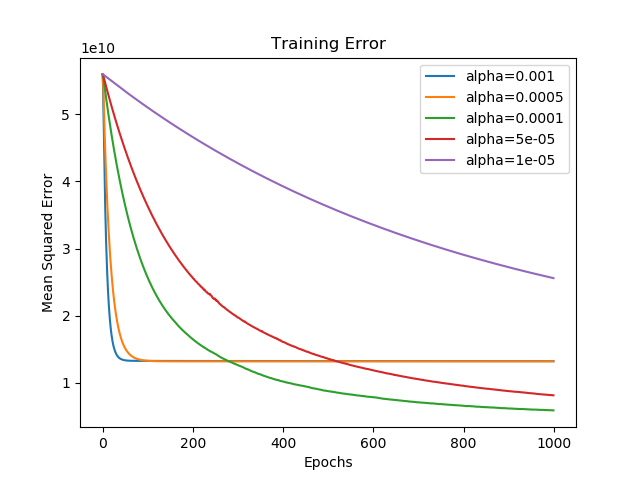
\includegraphics[width=\imgw]{images/p1b2_alpha_train.png}   
\end{center}

We decided to pick a learning rate of \(10^{-4}\) for the best accuracy.

Plotting the test errors against the number of epochs for the optimal
learning rate:

\begin{center}
    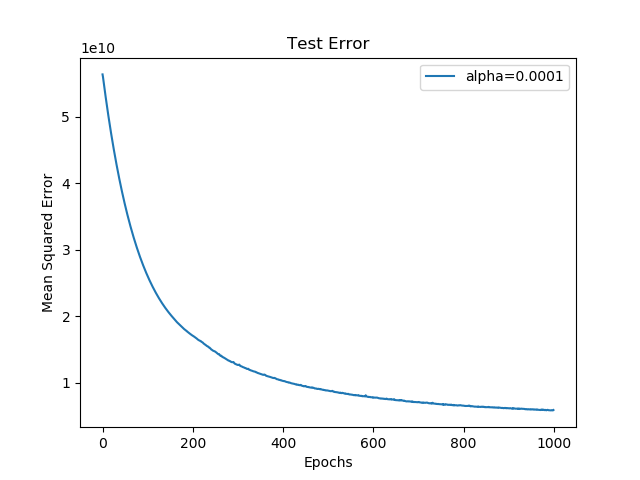
\includegraphics[width=\imgw]{images/p1b2_alpha_test.png}   
\end{center}

\subsection*{Experiment 3: Determining the optimal number of hidden neurons
(Question 3)}

The parameter \texttt{no\_hidden} is varied in the search space
\([20,30,40,50,60]\).
Plotting the training errors against the number of epochs for different
numbers of hidden neurons:

\begin{center}
    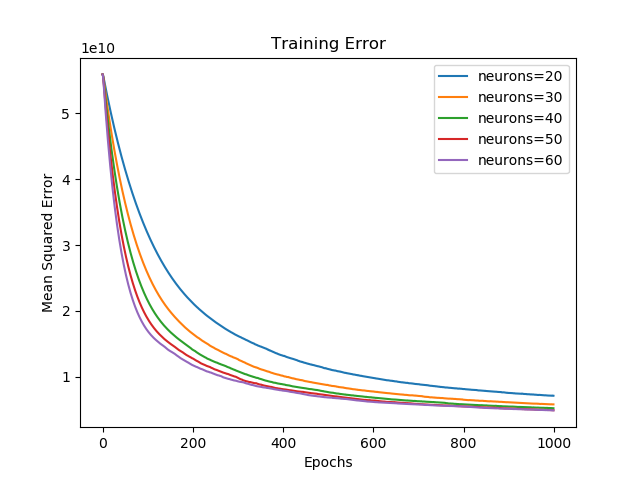
\includegraphics[width=\imgw]{images/p1b3_neuron_train.png}   
\end{center}

We decided to choose 60 hidden neurons for the best accuracy.

Plotting the test errors against the number of epochs for the optimal
number of hidden neurons:

\begin{center}
    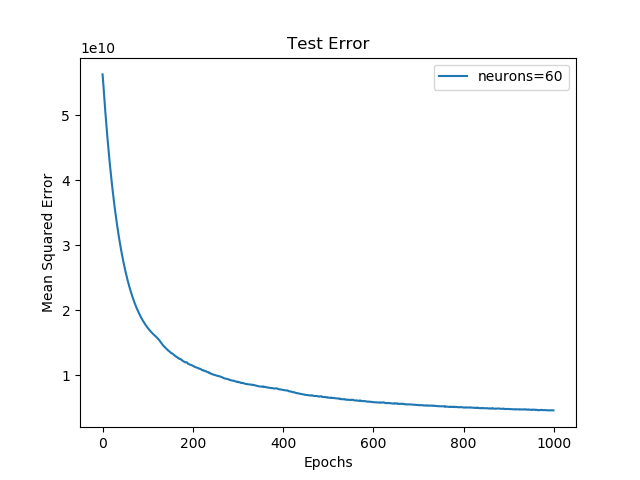
\includegraphics[width=\imgw]{images/p1b3_neuron_test.png}   
\end{center}

\subsection*{Experiment 4: The 4-layer and 5-layer neural network (Question 4)}

Plotting the test errors against the number of epochs for the 4-layer
network:

\begin{center}
    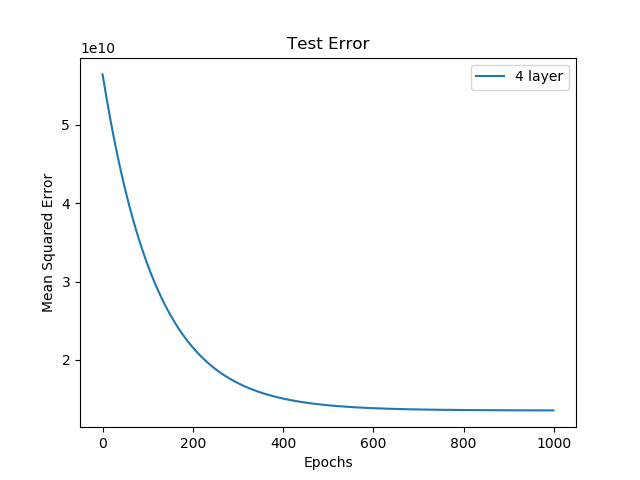
\includegraphics[width=\imgw]{images/p1b4_4layer_test.png}   
\end{center}

Plotting the test errors against the number of epochs for the 5-layer
network:

\begin{center}
    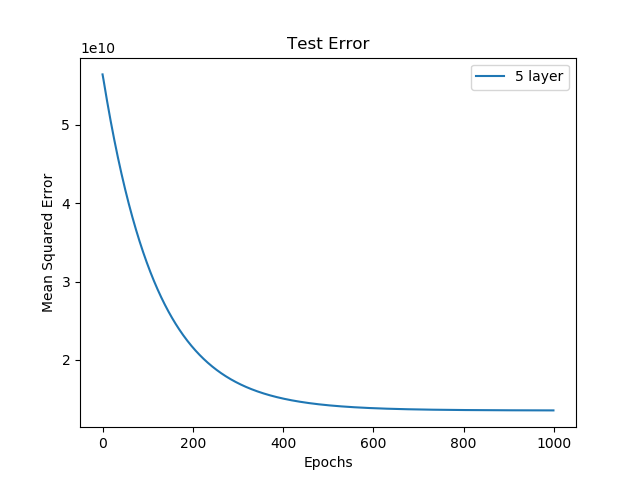
\includegraphics[width=\imgw]{images/p1b4_5layer_test.png}   
\end{center}

Comparing the performance of the 4 and 5-layer networks with the 3-layer
network:

\begin{center}
    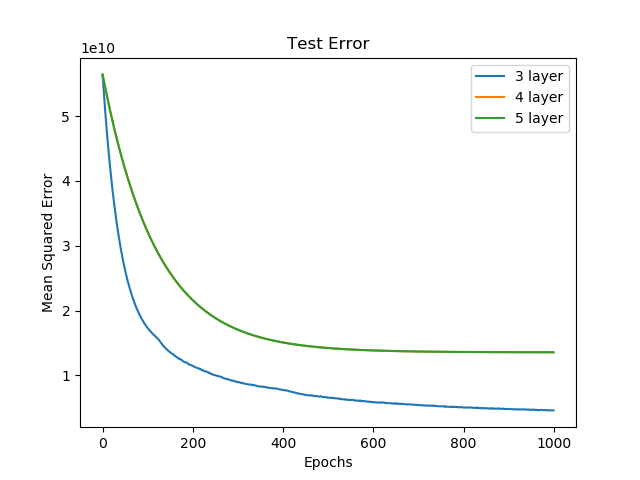
\includegraphics[width=\imgw]{images/p1b4_compare.png}
\end{center}

Note that the plots for the 4-layer and 5-layer networks
overlaps on each other.

The 3-layer network achieves a higher accuracy compared to the 4-layer
and 5-layer networks. This shows a similar result to the classification task,
where more layers do not neccesarily lead to higher performance.
